
\documentclass[brazilian,12pt,a4paper,final]{article}

%% Pacotes extras (opcionais):

% *babel* contem as regras de hifenização
\usepackage[portuguese]{babel}
% *t1enc* permite o reconhecimento dos acentos inseridos com o teclado
\usepackage{t1enc}

% *inputenc* com opção *utf8* permite reconhecimento dos caracteres com codificação UTF8, que é padrão dos esditores de texto no Linux. Isso permite reconhecimento automático de acentuação.
%\usepackage[utf8]{inputenc}
\usepackage{epsfig}

% *graphicx* é para incluir figuras em formato eps 
\usepackage{graphicx} % para produzir PDF diretamente reescrever esta linha assim: \usepackage[pdftex]{graphicx}

% *color* fontes soloridas
\usepackage{color}
%%% fim do cabecalho %%%

\pagestyle{empty}
\title{Métodos Computacionais Aplicados à Biocomplexidade}
\author{Aluno: André Gustavo Dessoy Hubner - Matrícula: 00315569 \\ IF-UFRGS}

\begin{document}
	\maketitle
	
	\section{Introdu\c{c}\~ao} 
	% Aqui a Introdução \c{c} e \~a  é a forma standar  de escrever
	% carateres ASCII extendidos (acentos, etc), porem com o pacote t1enc
	% declarado acima podemos escrever diretamente ç em lugar d \c{c}, etc
	\indent 
	Este documento trata de um programa para a identificação de genes de DNA e de RNA em genomas
	de bacterias que foi criado de forma experimental usando Python.
	Aqui será exposto o racional por traś da metodologia usada, assim como diversos outros pontos que
	elucidam a utilidade de ferramentas desse tipo para a resolução de problemas da Biotecnologia
	envolvendo anotação de genomas
	
	\section{Metodologia}
	\subsection{Classe Genome, configuração e inicialização}
	\indent
	Primeiramente, foi criada uma classe chamada de \textit{Genome}, que é usada para conter informações
	importantes e levá-las aos diversos métodos da anotação de genoma, que também estão contidos nela. No
	método construtor desta classe (\_\_\_init\_\_\_), foram definidos sete parâmetros cujos valores passados 
	pelo usuário configurarão todo o funcionamento da anotação para a instância gerada. A partir da instância
	da classe Genome, então, basta rodar o método AnnotateGenome, que chamará todas os métodos envolvendo 
	o processo da anotação de genoma. Chamar métodos outros que este ocasionará em erro, uma vez que eles estão
	marcados como métodos privados justamente para que não haja funções sendo processadas em ordem errada. Uma 
	exceção é o método SearchRNAGenes, que pode ser chamado sozinho para realizar a busca apenas por genes de
	RNA.
	
	\vspace{0.5cm}
	
	Dos sete parâmetros supracitados, apenas um é obrigatório, sendo este o primeiro, em que é especificado o caminho
	do sistema de onde buscar o arquivo .fasta contendo a sequência do genoma a ser analisado. Devido ao projeto ser
	experimental, outros tipos de entrada resultarão em erro. A sequência do arquivo será então utilizada pelo método
	GetSequence, através de manipulação de arquivo e string básica de Python, para extrair apenas a sequência, sem as informações
	contidas na primeira linha, e armazená-la como um membro de instância. Os seis parâmetros opcionais, por sua vez, tem funções 
	conforme a seguinte tabela:
	
	\vspace{0.5cm}
		
	\begin{itemize}
		\item minProb: produto mínimo das probabilidades dos Boxes -10 e -35 em relação ao possível gene (ponto
						que será explicado em uma seção posterior), de forma que ele seja
						considerado como um gene candidato. Assim, é possível controlar o equilíbrio quantidade/qualidade
						dos candidatos utilizando este parâmetro. Padrão 0 (sem filtro).
						
		\item minSize: semelhantemente ao caso acima, controla a qualidade dos genes candidatos, porém filtrando-os pelo
						tamanho da sua sequência codificadora. Padrão 3 (tamanho do códon de início).
						
		\item includeRNAGenes : booleano que indica se serão buscados genes não só de DNA como de RNA também no método 
								AnnotateGenome. como todos os 3 parâmetros posteriores também estão envolvidos na busca
								de genes de RNA, se este parâmetro tiver o valor de "False", os três não terão nenhum efeito.
								Padrão False.
		\item  searchString : string que deve corresponder a um organismo o qual será utilizado para obter as sequências padrão
								de rRNA e tRNA para a busca dos mesmos na sequência de genoma da instância. A obtenção dessas 
								sequências padrão é uma funcionalidade experimental e é realizada por busca no banco de dados do NCBI
								, ocasionando um aumento significativo do tempo de processamento. Caso não seja especificada nenhuma string
								ou passada uma string vazia assim como por padrão, serão utilizadas sequências locais de Escherichia coli sem 
								realizar a busca por API, demandando assim muito menos tempo de processamento. Devido aos pontos acima
								, recomenda-se utilizar o padrão e não especificar nada neste parâmetro. No entanto, sabe-se que as sequências
								de tRNA e rRNA não são iguais entre os organismos, portanto a busca de genes de RNA utilizando padrões
								de organismos bastante diferentes não resultará em resultados significantes. Logo, a construção desta funcionalidade
								levou em mente esse problema, modelando uma forma experimental de resolvê-lo.
								Padrão string vazia, o que resulta em usar sequências armazenadas
								localmente de Escherichia coli.
								
		\item rnaGenesCutoff: inteiro que representa a distância mínima em nucleotídeos entre dois genes candidatos de rRNA ou de tRNA. Isto existe pois genes de RNA
							  não precisam iniciar com um códon de início, ou seja, não é possível estabelecer genes candidatos imediatamente conforme 
							  os três primeiros nucleotídeos (assim como é feito para genes de DNA), tornando também impossível ter um critério bom para 
							  todos os casos de onde começar a buscar o próximo candidato. Sua existência também se deve ao fato de genes semelhantes
							  serem muito prevalentes para valores abaixo de 30, tornando boa parte dos resultados redundantes. Tendo isso em vista, o valor
							  padrão foi estabelecido como 30.
							  
		\item rnaGenesMinScore inteiro usado como score mínimo de um gene de RNA para ser considerado como candidato, permitindo controlar a abordagem
								quantidade/qualidade para genes de RNA também. Padrão 0.
	\end{itemize}
								
	
		A figura 1 mostra um exemplo de instanciação da classe Genome, realizando logo após um anotação da sequência especificada buscando por genes de DNA 
		de tamanho mínimo de 3, produto das probabilidades de no mínimo 0.25, e genes de RNA com intervalo entre cada gene de no mínimo 30 nucleotídeos, com 
		score mínimo de 0,25 também e usando os padrões locais de Escherichia coli, conforme especificado no construtor da classe. Como já está implícito,
		o uso dessa abordagem permite fazer buscas com diferentes configurações.
		
		\vspace{0.5cm}
		
		O último ponto desta parte de configuração envolve a obtenção da sequência reversa da obtida no arquivo para obter também os genes de DNA possíveis
		 neste lado da fita de DNA. Isto é feito já no método AnnotateGenome, utilizando um dicionário contendo os reversos de cada nucleotídeo para obter uma
		 tabela de tradução, e então usando-a para converter a sequência primária na sequência reversa. Devido ao caráter experimental do projeto, a busca na fita
		 reversa só foi considerada para genes de DNA.
		 
		
	\begin{figure}[hbtp]
		\begin{center}
			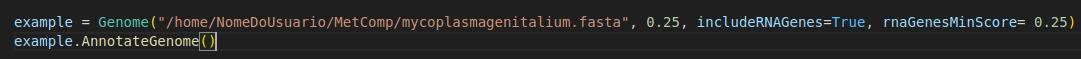
\includegraphics[]{Instanciacao.jpg}
			\caption{figura demonstrando a criação de uma instância da classe Genome e a realização da anotação do genoma por ela}
			\label{fig}
		\end{center}
	\end{figure}

		\subsection{Métodos essenciais na busca por genes de DNA}
	Para iniciar a busca de genes de DNA em dada sequência foi construído o método GetGene, que recebe a sequência alvo e um número n, buscando os genes a partir da
	n-ésima posição na sequência (considerando indexação baseada em 0). O ponto essencial dessa busca é que ela utiliza o método find de strings para, a partir de n,
	na sequência como string, buscar exatamente "ATG". Achado o primeiro ATG a partir de n, ocorrerá uma iteração de 3 em 3 nucleotídeos na sequência até achar um 
	códon de parada, parando então a busca e retornando o índice de início e o de fim do gene candidato. Caso não seja encontrado um ATG a partir de n, o valor retornado
	é -1, que é captado dentro do método para significar que a busca por genes de DNA acabou na sequência. Um ponto importante a considerar neste método foi que, devido
	ao genoma bacteriano ser circular, é possível que um gene comece perto da extremidade final do genoma (pelo menos considerando a representação em arquivo .fasta) e termine
	na extremidade de início ou até adiante. Para representar este ponto foi adicionado mais um laço de repetição no código, impedindo que um gene que comece no fim da string 
	seja cortado devido a ter chegado no "fim" da sequência.
	
	\vspace{0.5cm}
	
	Em seguida, atentando-se que em genes de bacterias existem duas regiões muito importantes para a transcrição da sequência, conhecidos como os TATA boxes -10 e -35 (justamente por estarem a posições de -10 e -35 nucleotídeos em relação ao início da sequência codificadora), foi feito um método para dar uma pontuação a uma certa sequencia de entrada
	para avaliá-la como um TATA box dependendo da sequência consenso do TATA box, que também é informada por entrada (parâmetro). O esquema de pontuação utilizado envolve, tendo como base um valor de 1, iterar por toda a sequência e, se o caractere atual for igual ao do consenso, multiplicar a pontuação pela porcentagem condizente ao nucleotídeo consenso naquela posição; caso contrário, a multiplicação ocorre com a probabilidade de não ser aquele nucleotídeo (\((1-p)/3\), considerando p como a probabilidade de ser o nucleotídeo consenso)
	pela sequência em questão.
	
	\vspace{0.5cm}
	
	Tanto GetGenes quanto GetPontuation são pontos fundamentais do programa, sendo executados iterativamente pelos métodos explicados na próxima subseção.
	A figura 2 mostra o funcionamento do primeiro método, enquanto que a figura 3 faz o mesmo para o segundo.
	
	\begin{figure}[hbtp]
		\begin{center}
			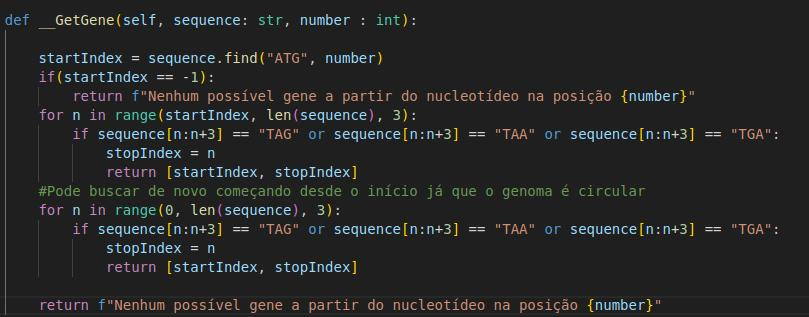
\includegraphics[]{GetGene.jpg}
			\caption{Busca da sequência codificadora de um possível gene, dado um genoma alvo e um número para começar a buscar, pelo método GetGene.}
			\label{fig}
		\end{center}
	\end{figure}

\begin{figure}[hbtp]
	\begin{center}
		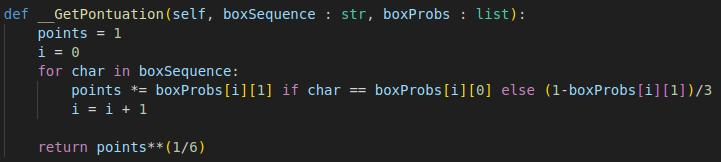
\includegraphics[]{GetPontuation.jpg}
		\caption{Atribuição da pontuação de uma sequência como TATA box para o padrão de box espećificado em boxProbs. boxProbs também deve conter as probabilidades associadas com cada nucleotídeo consenso, permitindo o cálculo da pontuação.}
		\label{fig}
	\end{center}
\end{figure}

\subsection{Busca iterativa de genes de DNA}
Dados os métodos construídos anteriormente, era necessário juntá-los em algo que percorresse o genoma inteiro. Primeiro, considerando um possível gene já achado, construiu-se o método GetBestBoxes que, recebendo um genoma e o a posição de início do gene achado neste genoma, retorna os boxes -10 e -35 de maior pontuação para o gene associado. Este passo é necessário uma vez que os TATA box não estão necessariamente a exatamente 10 e 35 nucleotídeos a montante do codon de início, na verdade, sabe-se que a distância entre o início e primeiro box pode ser de 6 a 10 nucleotídeos, enquanto que o outro box pode estar de 17 a 20 nucleotídeos de distância do box -10. Logo, a função deste método é justamente de buscar qual sequência de 6 nucleotídeos entre todas nessas posições tem a melhor pontuação para o respectivo TATA box, utilizando o método GetPontuation como descrito anteriormente. A implementação foi bastante condizente com a descrição acima, conforme demonstrado na figura 4. O método retorna uma lista contendo as pontuações dos melhores boxes -10 e -35, além de uma string representando todos os nucleotídeos do códon de início até o box -35, com uma representação logo abaixo dos melhores boxes identificados da respectiva sequência consenso utilizada.

\begin{figure}[hbtp]
	\begin{center}
		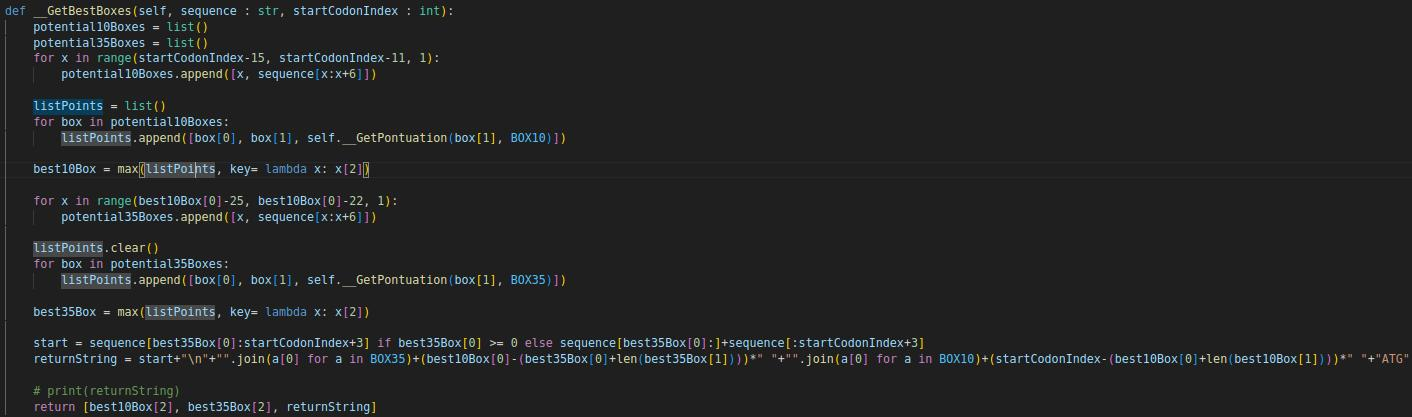
\includegraphics[]{GetBestBoxes.jpg}
		\caption{Método GetBestBoxes, que vasculha a região a montante do gene candidato encontrado, retornando as pontuações dos melhores boxes encontrados assim como uma representação em string da região.}
		\label{fig}
	\end{center}
\end{figure}
	
	
	\vspace{0.5cm}
Finalmente, o método FindGenes representou a junção de todas as peças desse quebra-cabeça. Recebendo o genoma alvo como string e uma lista onde serão armazenados os resultados, sua função é garantir a busca iterativa por genes no genoma especificado até que se chegue ao fim. No código isso ocorre dentro de um laço While com o argumento "True", especificando portanto que a iteração ocorra até que algo a impeça explicitamente. Logicamente o primeiro método a ser chamado é o GetGene, começando a busca pela posição 0, e então apenas se esse gene tiver o tamanho mínimo parametrizado na inicialização da instância se buscará pelos melhores boxes com GetBestBoxes. Por fim, se o produto das probabilidades dos boxes encontrado nesta última chamada for maior que probabilidade mínima dos parâmetros, adiciona-se esse gene, incluindo informaçoes relevantes retornadas pelos métodos anteriores, na lista para retorno. Independentemente de se o gene atual cumpriu as restrições dos parâmetros a busca por genes começa novamente a partir da posição de início deste gene, fluindo normalmente até que GetGene retorne uma string que será identificada pela função nativa isInstance, quebrando o laço While e retornando a lista com as informações dos genes identificados. Este método está representado na figura 5.

\vspace{0.5cm}

\begin{figure}[hbtp]
	\begin{center}
		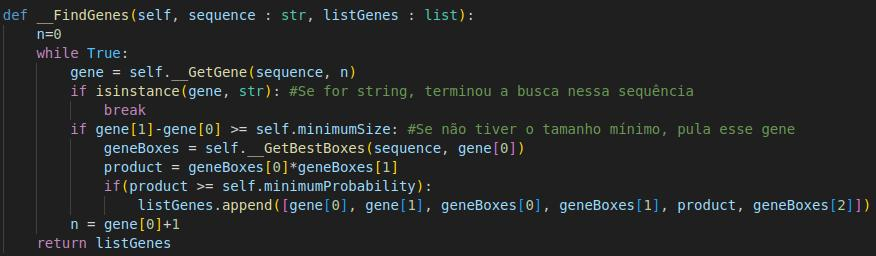
\includegraphics[]{FindGenes.jpg}
		\caption{Iteração por todo o genoma pesquisando por genes candidatos e retornando seus dados pelo método FindGenes}
		\label{fig}
	\end{center}
\end{figure}

Uma vez achados todos os genes possíveis para a fita forward do genoma, o mesmo processo se repetirá tendo como base o outro lado da fita, usando a sequência obtida através da tabela de tradução assim como descrito no fim da primeira subseção, e adicionando os novos candidatos à mesma lista de retorno.
No entanto, finalizada a busca por genes de RNA, começa a busca por genes de rRNA e de tRNA caso o usuário tenha passado includeRNAGenes como True.

\section{Busca de genes de rRNA e tRNA}
\subsection{Obtenção dos padrões e buscas no NCBI}
Novamente, devido ao caráter experimental do projeto, a busca de genes realizada aqui é de complexidade abaixo do que se veria em soluções reais com times dedicados. Dito isso, a solução aqui tentou aplicar conhecimentos difundidos sobre tRNAs e rRNAs para resolver o problema à mão. Isso é visto logo de início, pois antes de iniciar a busca por esses genes, pode-se buscar os padrões de 16S rRNA, 5S rRNA e 23S rRNA e de todos os tRNAs para o organismo específicado em "searchString", de forma a melhorar a qualidade dos resultados obtidos. 

\vspace{0.5cm}

Mais detalhadamente, essa busca ocorre nos métodos "GetrRNATemplate" e "GettRNAsTemplates", onde ocorre a busca pela sequência em questão de forma bem semelhante, acessando a conexão ao Entrez do Biopython, primeiro com uma função "esearch" onde se procura pelos resultados de uma pesquisa como se fosse feita na página do NCBI, tendo o banco de dados "nucleotide" como alvo, e abrindo o primeiro dos resultados com a função "efetch". A primeira função é chamada três vezes, uma vez para buscar cada rRNA, enquanto que a segunda chama 20 vezes a outra função "EntrezSearchtRNA", responsável só pela pesquisa no Entrez, e dentro dos resultados de cada uma delas armazena apenas aqueles que tiverem entre 100 e nucleotídeos, uma vez que se sabe que o tamanho de sequências codificadoras de tRNAs está próxima dos 78 nucleotídeos, para todos esses casos. Cada uma dessas funções está configurada para retornar uma exceção caso haja um erro na pesquisa, parando o fluxo de execução e retornando o erro encontrado.

\vspace{0.5cm}

Por outro lado, devido à complexidade que essa abordagem leva ao projeto, especialmente em termos de processamento, deve ser considerada como utilização padrão a de não especificar o parâmetro searchString, obtendo as sequências padrão desses RNAs para \textit{Escherichia coli}, que estão presentes no arquivo "Templates.py". A maioria dessas sequências por sua vez foram obtidas da mesma forma que seria feita pelas funções do parágrafo acima, pesquisando no NCBI, banco de dados "nucleotide", por "{x}S rRNA[Title] AND {y}[Orgn]", em que x é a númeração do rRNA e y o nome do organismo específicado em searchString, nos casos de rRNA, e "tRNA-{z}[Title] AND y[Orgn]", em que z é o aminoácido do tRNA e y o nome do organismo, para as buscas de tRNA. Contudo, nem para todos os tRNAs foi achada uma sequência dessa forma, sendo poucas delas obtidas no site "biocyc.org".

\subsection{Busca por genes de rRNA e tRNA}

O fluxo de execução do programa segue então a busca por genes de DNA e, terminada esta, começa a busca por genes de RNA chamando "SearchRNAGenes", que chamará os métodos especializados para cada tipo de RNA, SearchrRNAGenes e SearchtRNAGenes. A lógica do primeiro é praticamente idêntica à utilizada no método FindGene, tendo, para cada rRNA a ter candidatos buscados, um laço de repetição While marcado com True que chama um método para buscar um gene, parando a busca caso seja retornada uma string e adicionando o produto aos resultados caso ele tenha uma pontuação maior à do filtro que, neste caso, é o determinado pelo parâmetro rnaGenesMinScore. 

\vspace{0.5cm}

Uma limitação importante da heurística usada aqui é que não dá para saber
exatamente onde um possível gene começaria, buscando pelos "ATG"s assim como anteriormente. Embora aqui se considere sequências que comecem com três nucleotídeos iguais, isto é em referência aos três primeiros do padrão obtido nos passos anteriores do RNA, substituindo nucleotídeos inconvencionais (bastante presentes em genes de tRNA) por adenosina. Isto de fato é uma limitação bem grande, porém, considerando que durante a iteração serão encontrados vários candidatos (assumindo que seja usado um valor de cutoff para RNAs razoável) e o cálculo de semelhança ocorre percorrendo o mesmo número de nucleotídeos do padrão alvo, devem ser retornadas pelo menos algumas sequências com score significante. 

\vspace{0.5cm}

Na busca por genes de tRNA em SearchtRNAGenes, o padrão do laço de repetição também se repete, porém com algumas leves diferenças que exigem um método especializado. Primeiramente se garante que haverão 20 iterações pelo genoma, cada uma realizando a heurística para cada um dos tRNAs que transporta um aminoácido em específico, utilizando a lista "AMINOACIDS", declarada no início do arquivo, e, logo em seguida, prepara-se uma lista para armazenar os candidatos desse tRNA ao membro de instância tRNAsGenes. Este membro é um dicionário que conterá como chaves cada aminoácido e como valores dessas chaves os respectivos candidatos. Cada laço reaproveita o método GetRNAGene já explicado para realizar a busca e os filtro também de acordo com "rnaGenesMinScore".

\vspace{0.5cm}

Concluídos esses passos, termina-se também a chamada ao AnnotateGenome. As figuras 6 e 7 trazem imagens do código das buscas por CDSs de rRNA e tRNA, respectivamente. Após o fim desse método, pode-se usar então o método PrintResults para obter todos os resultados obtidos ordenadamente no terminal, assim como suas informações. No próximo passo, serão feitas análises estatísticas dos resultados obtidos por diferentes configurações, o que também validará as abordagens escolhidas.

\begin{figure}[hbtp]
	\begin{center}
		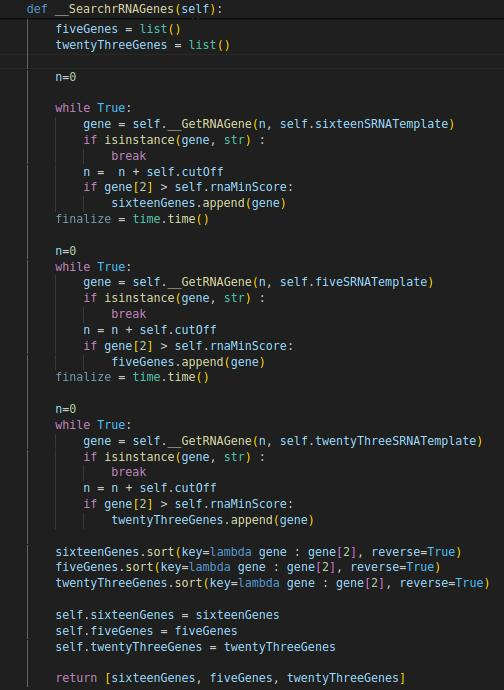
\includegraphics[]{SearchrRNAGenes.jpeg}
		\caption{Busca por todos os genes de rRNA, iterando uma vez pelo genoma para cada rRNA a ser buscado.}
		\label{fig}
	\end{center}
\end{figure}

\begin{figure}[hbtp]
	\begin{center}
		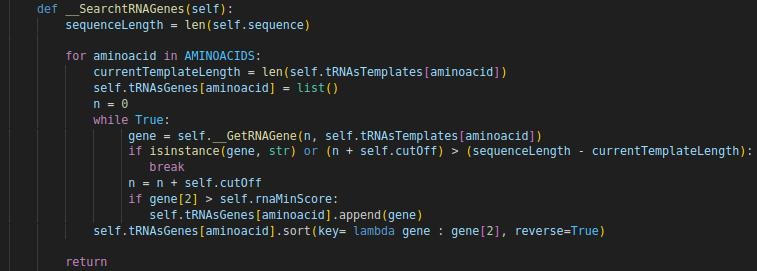
\includegraphics[]{SearchtRNAGenes.jpg}
		\caption{Busca por todos os genes de tRNA, iterando uma vez pelo genoma para cada tRNA a ser buscado.}
		\label{fig}
	\end{center}
\end{figure}


	
	
	
	
	\section{Resultados}
	\vspace{0.5cm}
	\subsection{Testando filtros de tamanho de CDS e probabilidade e dados gerais }
	Para as análises estatísticas envolvendo gráficos utilizou-se a biblioteca Matplotlib de Python, que já é bem estabelecida para análises deste perfil, em um arquivo separado chamado de "Análises estatísticas.py". Almejou-se medir o impacto do filtro de tamanho de CDS no número e qualidade dos possíveis genes de DNA obtidos na anotação de genoma, aproveitando para isso a chamada de AnnotateGenome em diferentes instâncias de Genome, tendo portanto os seus resultados disponíveis para fornecer como input nas funções de construção de gráfico do Matplotlib. 
	
	Para o primeiro gráfico, foram comparados dados de oito instâncias com diferentes filtros mínimos de tamanho de CDS. Dessas, a primeira atuava sem filtro, a segunda com tamanho mínimo de 30, a terceira de 100, a quarta de 300 e a partir de então cada instância tinha um filtro maior em 300 nucleotídeos até a última instância com tamanho mínimo de 1500 nucleotídeos.
	Tendo como pontos do eixo x o tamanho mínimo de cada instância e no eixo y o número de genes para cada um deles, plotou-se então um gráfico de barras, que pode ser observado na figura 8.
	
	Como é possível observar, de forma pouco surpreendente, filtros de tamanhos mínimos menores obteram bem mais genes candidatos, ao ponto que é difícil apontar um valor aproximado aos genes obtidos para as instâncias de filtros maiores. Por esse motivo, realizou-se outra plotagem, desta vez configurando o eixo y de forma que esteja em escala logarítmica e seus pontos marcados em cada valor exato de y, além de colocar retas ligando cada pontos. Com isso, obteve-se o segundo gráfico na figura 8, que demonstra uma tendência de redução dos genes obtidos praticamente logarítmica conforme se aumenta o CDS de acordo com os valores usados.
	
	Ainda para essas instâncias, calculou-se a média dos boxes de cada gene de cada instância, imprimindo-os ao terminal ao rodar esse arquivo. Nesses dados, observa-se que a distribuição das médias varia muito pouco, sendo as maiores e menores médias do box10 de 0.2635 (26,35\%) e 0.2516 (25,16\%), e do box35 de 0.2421 (24,21\%) e 0.2350(23,50\%), respectivamente, outro fato esperado, uma vez que a diferença do tamanho dos CDS não deveria afetar significativamente a qualidade dos candidatos obtidos.
	
	Já o próximo gráfico teve como objetivo verificar a funcionalidade do filtro de produto mínimo entre as probabilidades dos boxes 10 e 35, aproveitando também para saber a quantidade de genes para cada probabilidade que são retornados. Para isso, foram utilizados histogramas em que o eixo x representa uma faixa de probabilidades do box 10 ou 35, enquanto que o eixo y representa o número de genes encontrados para essa probabilidade nesse box. Para este estudo, foram escolhidas três instâncias : a primeira sendo sem filtro; a segunda com produto mínimo de 15\%, representando um filtro intermediário; e o terceiro com produto mínimo de 25\%, filtrando a maioria dos genes. Plotou-se portanto 6 gráficos, todos representados na figura 9.
	
	O primeira inferência clara que se pode a fazer é que filtros de valores maiores reduzem drasticamente a quantidade de resultados, sendo observados apenas 9 genes para o filtro de 25\%, ao passo que sem filtro são obtidos 15691 genes (visualizável na figura 8). A segunda é que, sem filtro, parece haver uma proeminência muito grande de genes com probabilidades dos boxes até 40\%, enquanto que nos gráficos dos filtros essa probabilidade parece estar em valores significativamente acima, com cerca de metade dos genes identificados estando em probabilidades de 40\% para cima usando o filtro de 15\%, e ainda mais para o filtro de 25\%, embora este último resultado possa não ser tão relevante estatísticamente devido ao número menor de genes encontrados. De fato, de acordo esses dados, usar valores maiores no parâmetro de produto de probabilidades mínimo aparenta ser uma forma eficiente de controlar rígidamente o equilíbrio entre qualidade e quantidade dos produtos a serem obtidos.
	
	Feita essa última análise, percebeu-se que ainda não se havia visualizado o número de genes obtidos por tamanho, aproveitando também para observar as diferenças nessas estatísticas entre os casos sem filtro, com tamanho mínimo de 600 e tamanho mínimo de 1500. Essa visualização está disponível novamente em formato de histograma, de acordo com a figura 10. Também foi realizado o cálculo do tamanho médio de cada uma dessas instâncias, obtendo os valores de aproximadamente 78, 1002 e 2004, seguindo a ordem anterior, denotando novamente o efeito esperado ao usar esse tipo de filtro. Com isso, foram finalizadas as análises para genes de DNA.
	
	\subsection{Resultados de rRNA, tRNA e do filtro de score de RNAs}
	A última seção, por sua parte, teve como intuito validar brevemente a abordagem utilizada na busca por genes de rRNA e tRNA no que tange o número de genes encontrados e o score deles. Para isso, tanto para genes de rRNA quanto de tRNA, foram usadas duas instâncias: a primeira percorrendo os métodos de RNA de forma padrão, apenas com o parâmetro "includeRNAGenes" assinalado; e a segunda contendo também o parâmetro "rnaGenesMinScore" com o valor 0.25.
	
	Tendo isso em vista, primeiro realizou-se a plotagem dos dados de rRNA, em que cada linha dispõe os dados de um dos rRNAs buscados e cada coluna determina se diz respeito à busca com ou sem filtro. Foi possível assim obter a figura 11, onde o fato mais notável é que curiosamente os dados da ocorrência sem filtro apresentam-se num padrão de distribuição normal. Isso, contudo, não é nada fora do comum e realmente esperado, uma vez que o genoma analisado neste projeto é da bacteria \textit{Mycoplasma genitalium}, cujo gênero é bastante idiossincrático, conhecido por ter vários dos organismos com os menores genomas conhecidos e possuindo padrões de metabolismo bastante diferentes devido a essa limitação. Logo, sem dúvidas é um organismo bastante diferente de \textit{Escherichia coli}, organismo base de todas as sequências padrão utilizadas para obter o score, sendo estas consequentemente razoavelmente diferentes das sequências que foram analisadas na busca aqui. A princípio seriam feitas mais análises com dados trazidos de uma busca usando um valor de "searchString" tendo como alvo esse organismo, porém como não é possível obter todas as suas sequências em buscas ao NCBI conforme implementado aqui, isto foi descartado.
	
	
	
	
	
	
	
	
	
	  
	
	\indent 
	Primeiramente desejou-se obter a sequência sem quebras de linha, deixando ela mais limpa.
	Para isso, o arquivo "Pkc1p\_saccharomyces.fasta" foi aberto em formato de leitura e armazenado
	em uma variável, a qual foi usada então para ler todas as linhas na variável "texts" e, para cada
	linha dessa variável, tirar caracteres especiais como os \textbackslash{}n com a função "strip()", armazenando 
	então na variável "sequence". Logo em seguida essa sequência inteiramente convertida para RNA foi
	armazenada na variável "mRNASequence". Esses resultados estão expostos na figura 1:
	\vspace{0.5cm}
	
	\begin{figure}[hbtp]
		\begin{center}
			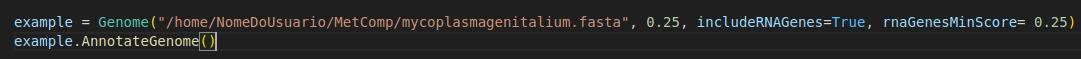
\includegraphics[]{Instanciacao.jpg}
			\caption{figura demonstrando a leitura da sequência e sua conversão para RNA}
			\label{fig}
		\end{center}
	\end{figure}
	
	\subsection{Análise das sequências}
	O próximo passo consistiu de análises básicas sobre a sequência de DNA. Primeiramente foi obtido o número de nucleotídeos ao começar a buscar na sequência a partir do primeiro ATG, que indica o início da sequência a ser transcrita e obtendo o seu tamanho com a função
	len(). Após isso foi possível obter facilmente as quantidades de cada nucleotídeo, assim como de sequências de "GC" e "AT", utilizando a função count().
	
	Assim, obteve-se 1197 adenosinas, 918 timinas, 693 guaninas e 648 citosinas, 125 sequências de GC, 306 de AT e uma porcentagem de GC de 38,80. A figura 2 mostra o código executado para obter cada um desses dados.
	
	
	\subsection{Código genético e tradução para proteína}
	As próximas questões envolveram a tradução do mRNA desse gene para sequência de aminoácidos e o código genético que permite isso. Os codons do mRNA foram obtidos ao primeiro obter a sequência pura de mRNA e então adicionando a uma lista cada sequência de três nucleotídeos contidos nela até o fim.
	
	Para a tradução, no entanto, foi necessário obter primeiro o índice do codon de parada para então obter a sequência que seria traduzida de fato. Isso foi feito iterando pela sequência pura até encontrar um dos códons UAA, UAG ou UGA, conhecidos como códons de parada, e armazenando na variável sequenceToBeTranslated.
	
	Finalmente então foi possível obter o número de aminoácidos que seriam traduzidos \textit{a priori} dividindo o seu tamanho por três e aplicando a função floor() (para caso a sequência não seja múltipla de três), e traduzir de fato a sequência . Isto foi feito iterando a passos de três pela variável sequenceToBeTranslated e, se é possível pegar a próxima sequência de tamanho três (ou seja, ainda não terminou a sequência a ser traduzida)  pegando a partir do dicionário que contém o código genético o aminoácido correspondente a ela e adicionando-o à nova string translatedSequence.
	
	A contagem de aminoácidos \textit{a priori} e \textit{a posteriori} foi de 1151 e a sequência de aminoácidos obtida começa em metionina (codificado pelo códon de início) e termina em leucina que é codificada pelo códon UUA, o último antes do códon de parada \textit{in-frame} UGA que é possível identificar no final da sequência. Logo, a tradução é bem validada. O código correspondente a esta seção se encontra nas figuras de 3 a 5.
	
	
	\subsection{Análises com a sequência de aminoácidos}
	O último passo foi realizar análises básicas da sequência de aminoácidos obtida da tradução. Primeiramente foram calculadas as quantidades de histidina (H) e serina (S), e a porcentagem de triptofano (W), sendo estes 30, 86 e 1,12\%, respectivamente.
	
	Em seguida, para calcular as porcentagens de todos os aminoácidos na amostra se calculou o conjunto de todos os aminoácidos a partir do dicionário do código genético com a função set() e retirando os códons de parada, uma vez que eles são apenas de parada e não costumam trazer um aminoácido à proteína resultante. Então, para cada um desses aminoácidos, adicionou-se à lista aminoacidsPercents um array contendo ele e a porcentagem dele na amostra.
	
	Essa lista já contém todos os dados necessários, mais ainda era necessário ordenar ela. Para isso se usou a função sort() para ordenar primeiramente pela porcentagem e depois pela ordem alfabética da letra que representa o aminoácido através da função itemgetter(), e em ordem reversa especificada por reverse=True. Após isso esses dados foram exportados para CSV para serem analisados por meio do Gnuplot.
	
	No Gnuplot então, foi possível gerar um histograma que representa fielmente as porcentagens obtidas utilizando o estilo de dados "histograms". O código desta seção e o gráfico correspondente no gnuplot se encontram nas figuras 6 e 7, respectivamente.
	
	
	
	\section{Conclusões}
	Foi possível, portanto, realizar todo o fluxo DNA -> RNA -> Proteína com a amostra de DNA de forma fiel tendo em vista os resultados das análises obtidas. Análises deste tipo podem ser expandidas para analisar as sequências codificadoras de várias proteínas, e de fato podem ser úteis para reconhecer padrões em DNAs, mRNAs e proteínas e identificar a função do produto de codificação, ou sítios de interesse nessas sequências, entre outras possibilidades.
	
	
\end{document}

